\chapter{Experiments and Results}\label{ch:experiments}
This section will present the experiments carried out in the different parts of SemReBot2 as well as a full system test. For a discussion around the results, see Section \ref{ch:discussion}. The experiments aim to highlight the advantages and disadvantages of the different model sizes, and each subsection will present the key findings for each part of SemReBot2. A full description of the test sets and results can be found in Appendix \textcolor{red}{X}. 

The experiments are primarily targeted at the specific use case of SemReBot2. Creators of models and packages used in SemReBot2 have conducted their own experiments for general purpose use, and the reader is encouraged to read the official papers of Whisper\cite{radford_robust_2022}, Mistral\cite{jiang_mistral_2023}, POPF\cite{coles_forward-chaining_2021} and PlanSys2\cite{martin_plansys2_2021} respectively for general performance experiment results.

\section{Whisper}\label{sec:Whisper_experiments}
The experiments conducted on Whisper were performed to compare the performance of different model sizes and to determine whether loading models with flash attention increased or decreased performance. The chosen metrics were WER, RTF, allocated memory during inference, and inference time.

The test set consists of ten audio files with a corresponding reference text. The audio files are news segments with a duration of 123 seconds to 824 seconds downloaded from Rev.com\cite{revcom_transcript_2024}, accompanied by a transcribed text.

The key results can be seen in Figure \ref{fig:whisper_avg}.

\begin{figure}[ht]
    \centering
    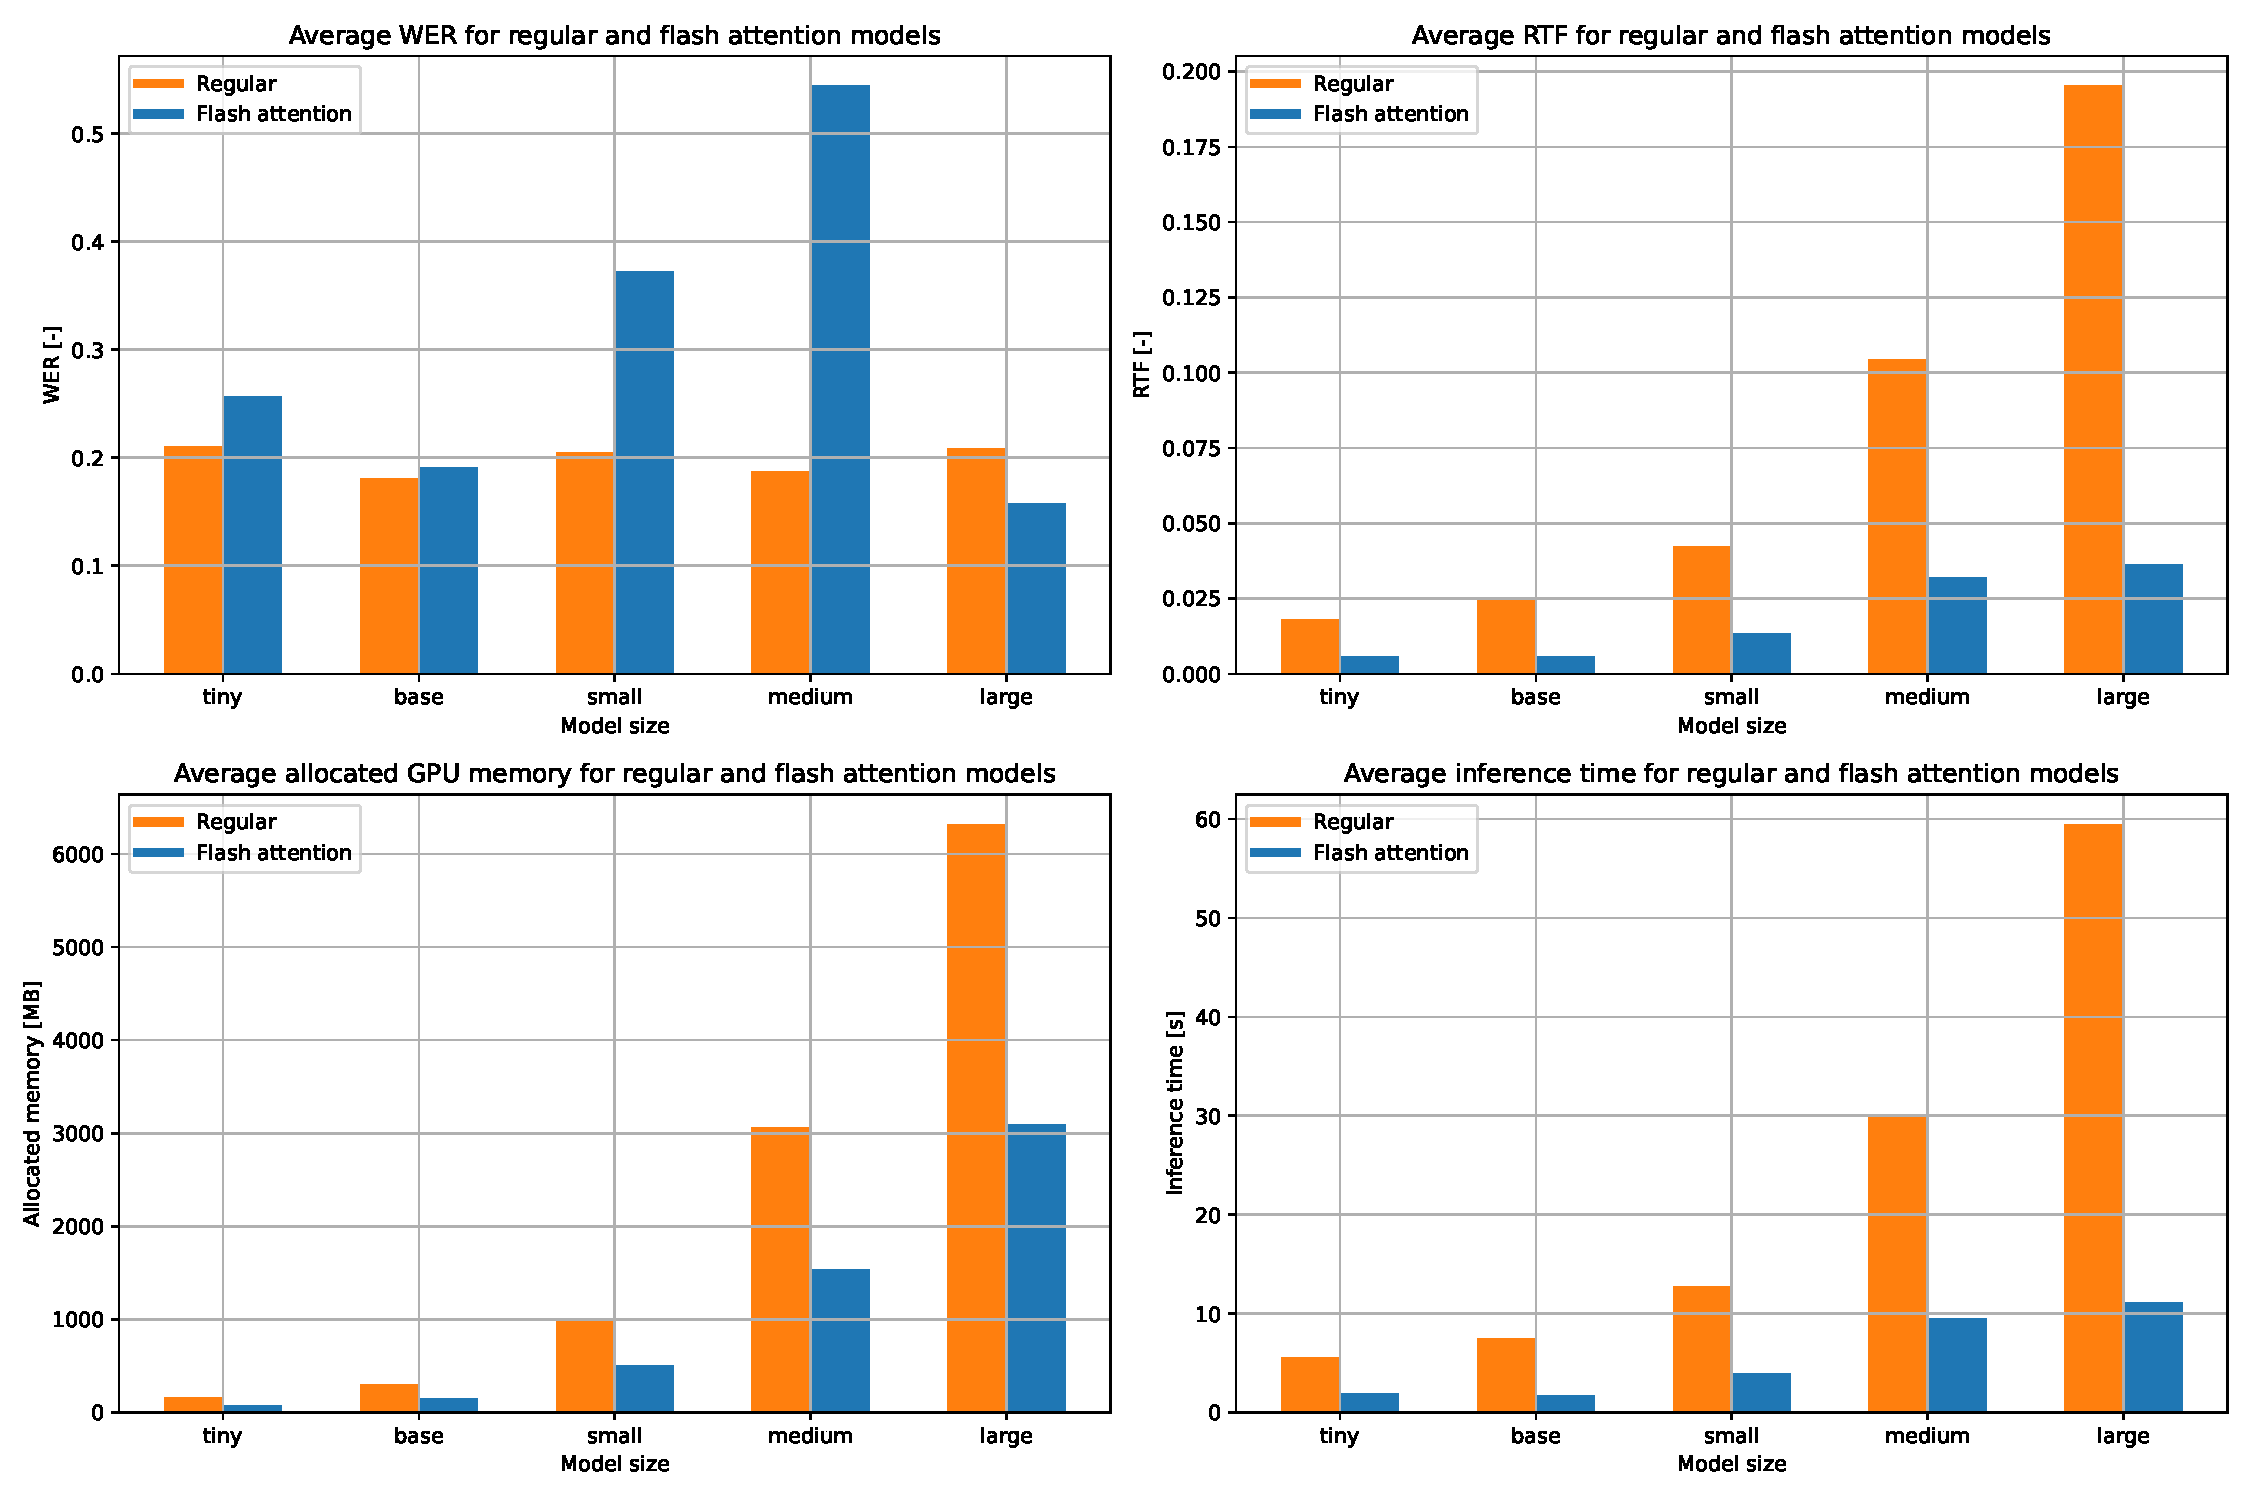
\includegraphics[width=\textwidth]{figures/avg.pdf}
    \caption[Whisper experiment results]{Comparison of Whisper model sizes loaded with flash attention and not. Measured metrics are WER (top left), RTF (top right), allocated memory during inference (bottom left) and average inference time (bottom right).}
    \label{fig:whisper_avg}
\end{figure}

\section{Mistral}\label{sec:Mistral_experiments}
Experiments conducted on Mistral were specific to the PDDL domain and the desired output format used in SemReBot2. We created two test sets where Mistral was given a PDDL domain with types and predicates available, as well as a natural language command.

\subsection{Test sets}
In test set 1, containing ten elements, each element consists of a domain extracted from the Github repository \verb|pddl-generators| by AI-Planning community\cite{favorito_ai-planningpddl-generators_2024}\footnote{This repository contain domains and problems used to generate benchmarks for the International Planning Competition.}. We then accompany each domain with a natural language command and a solution containing the correct instances, predicates, and goals in the correct format as SemReBot2 expects. An element of test set 1 can be seen in Listing \ref{lst:elem_test_set_1}

In test set 2, all eleven elements contain the same PDDL domain, which is the same domain as in the simulated environment, but different accompanying natural language commands and solutions. This test set is specific to the SemReBot2 use case.

\begin{lstlisting}[caption={An element of test set 1 showing the domain and command Mistral is given. The output is to measure if Mistral is correct or wrong.}, label=lst:elem_test_set_1]
{
"domain":"(:types worker task location)
          (:predicates (available ?worker - worker)
          (assigned ?task - task ?worker - worker)
          (located ?task - task ?location - location)
          (completed ?task - task))",
"command":"Assign the new tasks to workers efficiently. Task1 is at
           Location1, Task2 at Location2.
           Worker1 starts available.",
"solution":"instance worker1 worker|instance task1 task|
            instance task2 task|instance location1 location|
            instance location2 location|predicate available worker1|
            predicate located task1 location1|
            predicate located task2 location2|
            goal assigned task1 worker1|goal assigned task2 worker1|"
},
           
\end{lstlisting}

\subsection{Shot sets}
For each test set, we created one or two sets that we call "shot sets".

For test set 1, we created two shot sets, shot set 1 and shot set 2, with PDDL domains from \verb|pddl-generators| (but not the same as in test set 1), containing 32 elements with an accompanying natural language command and an output. The difference between shot set 1 and shot set 2 is that shot set 1 is unlabelled, while shot set 2 is labelled. That is, all the outputs in shot set 1 are correct, while every other output in shot set 2 is correct or wrong. So, shot set 2 contains an extra marker \verb|label| which is either \verb|correct| or \verb|wrong|. An element of shot set 2 can be seen in Listing \ref{lst:elem_shot_set_2}.

For test set 2, we used the same shot set as test set. However, if Mistral was running a test on element \verb|i| in test set 2, the shot set would contain all the previous elements in test set 2 as shots. This means that shot set 3 contain ten elements (\verb|len(test_set_2) - 1|).

\begin{lstlisting}[caption={An element of shot set 2. Notice the "label" marker. The output is wrong due to the text before first instance.}, label=lst:elem_shot_set_2]
{
"domain": "(:types portable location)
           (:predicates (at ?y - portable ?x - location)
           (in ?x - portable) (is-at ?x - location)) ",
"input":"Transport all the four objects to their respective location:
         first object to location 3, second object to location 0,
         third object to location 1 and fourth object at location 2.
         Also, go to location 1 afterwards. The four objects are now
         at location 3, location 1, location 2 and location 0
         respectively. We are in location 4.",
"output":"Here are the instances, predicates and goals:
          instance l0 location|instance l1 location|
          instance l2 location|instance l3 location|
          instance l4 location|instance o0 portable|
          instance o1 portable|instance o2 portable|
          instance o3 portable|predicate at o0 l3|
          predicate at o1 l1|predicate at o2 l2|predicate at o3 l0|
          predicate is-at l4|goal at o0 l3|goal at o1 l0|
          goal at o2 l1|goal at o3 l2|goal is-at l1|",
"label":"wrong"
},
\end{lstlisting}

\subsection{System prompts}
For all the tests that we ran, we created three different system prompts. A system prompt represents a chat history between a user and the assistant (read Mistral). All three system prompts explain what role Mistral has, its goal, and show one example of domain, natural language command, and expected output. The difference between the three is the length and the amount of detail Mistral is given. The prompts range between what we call "short and precise", "medium detailed", and "long and detailed". Listing \ref{lst:mistral_system_prompt} shows the short and precise system prompt.

\begin{lstlisting}[caption={The short and precise system prompt. domains[0], inputs[0] and outputs[0] is the first element from the shot set.}, label=lst:mistral_system_prompt]
system_prompt = """

As a PDDL assistant, your task is to outline the available instances,
predicates, and goals based on the provided domain and command.
Answer in the format shown after ### Output ###.

"""

message = [

{'role': 'user', 'content': system_prompt + f' Here is a domain:
                            {domains[0]}, and command {inputs[0]}.
                            ### Output ### {outputs[0]}.'},
                            
{'role': 'assistant', 'content': 'Understood.
                            Awaiting new domain and command.'},
                            
],
\end{lstlisting}

\subsection{Tests}
The first test was performed to see performance differences between a fine-tuned model for "SemReBot2 use" and zero-, one-, and few-shot prompting.

\subsection{Fine-tuned model}

\subsection{Pre-prompted model}
For the pre-prompted model tests, we ran three different tests:

\begin{itemize}
    \item Generic PDDL domain without labels
    \item Generic PDDL domain with labels
    \item Specific PDDL domain without labels
\end{itemize}

Every test was set up the same way: We first load the model into memory, extract one element from the test set, extract zero or more elements from the shot set depending on the number of iterations, run inference, and record the output before writing it to a file for storage. For all elements in a test set, we ran through all the elements in a shot set. This means that we recorded \verb|len(test_set)*len(shot_set)| number of test runs for each test set. We ensured that there was no information from previous test runs in Mistral by deleting and reloading the model before every inference run. See Appendix \textcolor{red}{X} for the model parameters used during the testing.

\begin{algorithm}\label{alg:mistral_test}
    \caption{Testing Mistral}
    \begin{algorithmic}[1]
        \State Load shot set, test set and system prompts
        \For{\textbf{each} test \textbf{in} test set}
            \For{\textbf{each} system prompt \textbf{in} system prompts}
                \For{\textbf{each} shot \textbf{in} shot set}
                    \State messages := system prompt + shot + test
                    \State Load model into memory
                    \State Perform model inference on messages
                    \State Write metric results to file
                    \State Delete model from memory and release resources
                \EndFor
            \EndFor
        \EndFor
    \end{algorithmic}
\end{algorithm}

In all tests, we measured inference time, allocated GPU memory during inference, model input size, and the output from Mistral compared to the solution. The output is compared to the solution by its accuracy in predicting correct amount of instances, predicates, and goals based on the domain and natural language command. The evaluation metric is subdivided into four distinct categories: $accuracy_{instances}$, $accuracy_{predicates}$, $accuracy_{goals}$ and $accuracy_{total}$.

\begin{equation}\label{eq:mistral_accuracy_metric}
    accuracy_{type}(\text{domain}, \text{command})=
    \begin{cases}
        1 & \text{if } output_{type} = solution_{type} \\
        0 & \text{otherwise}
    \end{cases}
\end{equation}

As seen in Equation \ref{eq:mistral_accuracy_metric}, each category, except for $accuracy_{total}$, employs a binary classification approach, in which the precision is deemed "correct" iff the output is exactly like the solution, disregarding variations in variable names. The total accuracy is then defined as

\begin{equation}\label{eq:mistral_total_accuracy_metric}
    accuracy_{total}=accuracy_{instances}\times accuracy_{predicates}\times accuracy_{goals}
\end{equation}

\section{POPF}\label{sec:POPF_experiments}

\section{SemReBot2 full system tests}\label{sec:SemReBot2_experiments}
Hei, fungerer dette? Jeg vet ikke, men vi sjekker.
\begin{equation}
    \frac{\alpha}{\beta} = \gamma
\end{equation}